\chapter{Your organisation is its tasks}
\addcontentsline{toc}{chapterdescription}{The whole point of any organisation is to deliver useful results by executing tasks or turning human energy into business output. How you do this depends on meaning\hyp{}making stories, matching the individual Size of Person with the Size of Role. Do this poorly at the leadership team level, and you suffer from a developmentally divided team; do it well and you’ll thrive. Whether you use sociocracy, Holacracy, Agile, or anything of that ilk, they all need developmental approaches and a FairShares Commons style incorporation to work.}
\addcontentsline{toc}{chapterdescription}{\pagebreak}
\label{chapter:who-is-your-organisation-tasks}


\begin{chapterquotation}
Chaos is found in greatest abundance wherever order is being sought. It always defeats order, because it is better organised.\\
\raggedleft\textemdash Terry Pratchett. \emph{Thief of Time}\index{Pratchett, Terry}
\end{chapterquotation}


\label{section:task-role-arena}


This chapter has been written to complement whichever of the many excellent sources you choose to use to approach organisation design, such as sociocracy or Holacracy. I have given the collective name of Ocracy to refer to the multiple practical implementations that have emerged from the philosophy of Auguste Comte in a neutral way that recognises the enormous value of any approach that enables a community of people to self-manage, self-govern or self-organise; and to emphasise the huge common ground they all share.  \index{Comte, Auguste}


In the previous two sections, we've looked through the lens of organisations as living, meaning\hyp{}making communities of living, meaning\hyp{}making individuals. This lens\index{lens} enables us to see clearly the physical and psychological human energy that is converted into business results. 


Energy\index{energy} is the most important element of an organisation to understand, if you need to improve performance, or the capacity for regeneration. 


There are only a few types of organisation forms common today. You have the classic  dictatorial hierarchy; the common organisational pyramid, which in larger organisations becomes a matrixed pyramid; a few flat teams without any hierarchy; and fewer self-organising flex-flow teams, which have a functional hierarchy that changes according to the immediate work context. Those of you familiar with the Spiral Dynamics\cite{beck-SD} \index{Spiral Dynamics} classification of worldviews, value systems, and the associated organisation designs, summarised in Table~\ref{table:SDi}, will recognise these. Spiral Dynamics \index{Spiral Dynamics} \index{Spiral Dynamics} is an excellent model and well worth gaining some familiarity in. Note that there are differences between the original of Beck and Cowan\cite{beck-SD} and the Spiral Dynamics Integral that combines it with Wilber’s\index{Wilber, Ken} integral work\cite{wilber-integral}.


\begin{table}[htbp]
        \footnotesize
        \begin{tabular}{ R{0.02\textwidth} L{0.15\textwidth}  p{0.12\textwidth}  p{0.12\textwidth}  L{0.40\textwidth} }
                \toprule
                \centering  &    &    SD & SDi & Characteristics \\ 
                \midrule
                {\large 8} & Holistic self & Turquoise & Turquoise & Focus on collective individualism, holding a multiplicity of perspectives, navigating a world with inherently nebulous, unknowable elements.\\
                \addlinespace[.1em]
                {\large 7} & Integral self & Yellow & Teal & Awareness of oneself within the world and cosmos. Integrate all layers 1-6, embracing functional hierarchies, focus on achieving needs through balance and development. \\
                \addlinespace[.1em]
                {\large 6} & Sensitive self & Green & Green & Social democracy, pluralism, belonging to a caring community, power with, human rights, dialogue and consensus, emphasise the group needs over own needs\\
                \addlinespace[.1em]
                {\large 5}& Rational self & Orange & Orange & Drive-strive, each individually plays the game to win, rationalism, meritocracy, market-driven. Focus on materialism and civilisation.\\
                \addlinespace[.1em]
                {\large 4}& Bureaucratic self & Blue & Amber & Order and purpose keeps everyone safe, there’s one right way to fit in, follow the rules, position not person hierarchies, discipline, inner stability, and faith will lead us to live well together and have good lives.\\
                \addlinespace[.1em]
                {\large 3 }& Power self & Red & Red & Power is what matters, do and take what you need through power, find and keep your place in the pecking order, focus on being a hero, power, glory, and revenge. Sacrifices to the power gods. \\
                \addlinespace[.1em]
                {\large 2 }& Magic, animistic self & Purple & Magenta & Egocentric, impulsive, magical thinking, a focus on placating the spirits. Wisdom of the elders, ancestors, of myths, and spirits. \\
                \addlinespace[.1em]
                {\large 1 }& Instinctive self & Beige & Infra-red & Survival. Narcissistic. Focus on basic needs. Catastrophe thinking. Use whatever strategies work, regardless.\\
                \bottomrule
        \end{tabular} 
        \caption[Overview of Spiral Dynamics]{ Brief overview of Spiral Dynamics \index{Spiral Dynamics}, with the colour schemes of Beck and Cowan’s original model in column SD, and Spiral Dynamics combined with Integral theory of Beck and Wilber in column SDi. }
        \label{table:SDi}
\end{table}


No organisational form is absolutely better or worse than any other, and each is ideally suited to certain types of challenges. For example, the dictatorial hierarchy can be the best organisational form if you have a small team dealing with the tasks of a technical crisis over a very short timeline; if you wake up in the dark at 3AM to discover that your house is on fire, for instance.


The classic pyramid and matrix organisations are only good at the roles and tasks of standardised production and iterative improvements.


The approach that’s best suited to delivering excellent results against large scale adaptive challenges is a flex-flow organisation design. 


For any organisation to be fully adaptive, it needs to have a flex-flow approach to roles and tasks, be excellent at mining and refining conflict\index{conflict} to regenerate all human capitals, and of course be incorporated to support both of those. 


\section{Where your organisation is: tasks}
\label{section:where-is-your-organisation-tasks}


I, (Graham), have developed, together with Bernhard Possert,\index{Possert, Bernhard} a classification scheme and diagnostic to evaluate where your organisation is on a scale from zero, dictatorial micromanagement, to autopoietic. 


Category zero, dictatorial, is definitely a dictatorial hierarchy; categories~4 and~5 are definitely flex-flow. The middle ones build a fluid bridge from the classic pyramid to flex-flow.


\begin{description}
\item[5 Autopoietic.] \index{autopoiesis} 
The external driver (context and need) that gives the organisation a purpose is what matters, not preserving the organisation for its own sake. The organisation is supported in gracefully dying by the rest of the ecosystem, especially all direct stakeholders, when the driver has changed beyond a level that the organisation can follow. 


The organisation\index{organisation} actively collaborates with other organisations in a larger ecosystem \index{ecosystem} (which may, for instance, be all the circles in a large-circle circular economy) in order to maximise the entire ecosystem’s capacity. The boundaries between organisations in the ecosystem, ecosystems, and stakeholders, are recognised as fluid and permeable. Everything is clearly recognised as multiple open nebulous systems in constant unpredictable and unknowable transformation. The inherent complementary pairing of competition and collaboration is a foundation of all business activities.


\item[4 Self-directing.]  
The budgeting process is flexible and continuous. Leadership can only step into autocratic decision power, limited to specific cases and clearly defined by the whole organisation, including at least staff, board, and investors, often with input from other stakeholders. 


Organisational strategy emerges through a cooperative process across the organisation, bottom-up and top-down. Teams decide for themselves who enters the team and who is ejected from the team involuntarily, individuals take decisions to move to another team after some form of consultation with their existing team. Most overhead functions and decisions occur within the teams. Roles, especially leadership roles, are filled by a democratic process.


\item[3 Self-governing.]  
Leadership, which may be in the form of an anchor circle, as found in the Ocracies,\index{Ocracy} focuses on a balance between the needs of individuals and the whole, spending time on systemic enablers that support self\hyp{}governing, interactivity, clarity, alignment, and direct coaching. 


Clear principles and rules for self-designing structures and processes are used to constantly and locally optimise the organisation for the immediate driver. Everybody can, and does, start a process without requiring permission from any hierarchy, to change any structures and processes to improve them and enable them to function well at work.


\item[2 Self-managing.]  
Everyone is aligned across the organisation, with the top-level strategies and central key performance indicators. The whole organisation has a common language about value and waste, which is used to increase value creation and minimise waste. 


There are common systems implemented to enable self-management of constellations of roles and the teams that fill them. Each individual has clearly defined roles including clear decision domains and clarity and authority on decisions within those domains. Teams\index{teams} manage and distribute their work themselves, not looking to a formal hierarchical boss to do it. Everything is structured in teams or circles.


\item[1 Delegated authority.]  
Experts are hired because they know things better than their bosses, and managers are comfortable with following the guidance of their expert direct reports, whilst retaining where necessary the decision authority on how to integrate the guidance across multiple domains of expertise in order to meet consumer needs and other business drivers. 


Project management systems are well implemented and practised, enabling different types of experts to collaborate and deliver results together. Individuals and teams define for themselves how to tackle the goals they are given. Each employee is seen as an expert within their role, and given an appropriate management for their expertise to be maximally useful to the organisation and to flourish.


\item[0 Dictatorial micro-management.]  
Employees are seen as inherently lazy, so their managers have to keep careful control of them, with powerful rewards and punishments, or they will stop working hard. Management, especially the CEO, is the only source of predictions about the future, and has sole accountability to generate detailed strategies and execution plans for the business to generate profit in that future. 


Management has all the power needed to exert sufficient control over all employees under them in the power hierarchy to keep them strictly executing the plan laid out by management; but if something turns out to be wrong at the end, it's then typically the employee’s fault, regardless. 


The boss always knows better, so even if you think you have a better solution, you keep quiet about it. People are not hired for thinking, so they should only act after their boss tells them what to do.
\end{description}


Where do you think your organisation is across these different categories? Most will find that they are spread out across a few. For example, if you are in category five, autopoietic, you will certainly have some of the best project management systems and practices around and score highly in Category~1.


The category you are most likely in, at any given moment, is your centre of gravity. You will recognise that you’re doing some characteristics from a higher category, but not sufficiently well, nor for sufficiently long, to regard that as a stable centre of gravity.


Equally, if your organisation has certain kinds of gaps in lower categories, you have foundations with weakness that may prevent you from succeeding, even though your organisation as a whole is striving upwards.


 Any more than occasional, limited elements of category zero indicate that your centre of gravity is still category zero, no matter how much you believe it is higher.


Keep in mind, if you are in a leadership position and use this as a frame of reference to evaluate where your company is, you are quite likely to put your organisation in a higher category than an external, anonymous, and unbiased controlled survey across all your staff.
\section{Requisite organisation design}
\index{requisite organisation design}
In Chapter~\ref{chapter:who-am-i-base} I described the never-ending process of how you can get to know who the ever-changing you is, across (1) how you think, (2) your stage of meaning\hyp{}making story, and (3) your fixed nature. In Section~\ref{section:size-of-person} we introduced all three of these together as your Size of Person (SOP).


In this chapter we have the Size of Role (SOR).\index{Size of Role} This is defined by the decisions requiring the most fluidity in how you think, the most complex stage of meaning\hyp{}making stories, and the greatest capacity to manage your nature and emotional state.


Elliott Jaques\index{Jaques, Elliott} observed over decades, both employed in organisations and as an academic, the characteristics of organisations that were highly successful in highly challenging business environments. He saw in them what he named requisite organisation design: designing organisations as human beings require them to be, in order for them to be able to perform at their best. Sadly he passed away in 2003, but his work lives on in the Requisite Organization Institute\footnote{\url{https://www.requisite.org/}}, \index{Requisite Organization Institute} co-founded with his wife and colleague, Kathryn Cason.\index{Cason, Kathryn}


In a requisite organisation everybody is in a role that is approximately the same size as they are: SOP~=~SOR. Neither the Size of Person nor the Size of Role should be too much bigger or smaller than the other. Otherwise, there will be problems.


If you are working in a role that is much smaller than your Size of Person, \index{Size of Person} one of two things will happen. Either you will get bored out of your mind, and end up suffering from bore-out, which is just as debilitating as burnout. (Both are becoming seen as work-induced depression.) Or, to avoid getting bored out of your mind, you will immediately set about increasing the complexity of your role until it is at least as big as you are, and gives you the challenge you need to be at peak performance.


Your organisation will suffer in both cases. If you increase your role’s complexity, you may well end up doing work that no one else in the team or even the organisation can follow, and may not even be meeting any of the current drivers. If you are the founder or the CEO, you will end up trying to lead your people, perhaps even your entire business concept, into places they are not yet ready to go. Quite likely your organisation will implode.


Equally, if your role is way too big for you, you are either going to end up burning out, as you valiantly try everything you can to cope single-handedly despite being in over your head, or you will trim the role down to your size.


Again, in both cases, your organisation will suffer. If you burn out, you will be underperforming for however long it takes before you and your organisation realise what is happening, and for the time it takes for you to heal. You may well be out of action for many months and still cost your organisation your fully loaded employee cost. You may find that you carry the scars of burning out for the rest of your life and that your career is never what it would have been if your manager, or lead link in a self-governing circle, had never put you into a role too big for you. 


In the worst case, no one, not even you, recognises that this is not your problem, but rather, it is work-induced depression caused by your management allocating you to a role way bigger than your Size of Person. \index{Size of Person} In this case, you will likely blame yourself, absolving the manager or lead link of all accountability, and simply accept being fired for poor performance, or resign in a depression. 


In the worst case, this can lead to employees dying by their own hand\footnote{The nonprofit Minds at Work \index{Minds at Work} in the UK was founded by Geoff McDonald, \index{McDonald, Geoff} former Unilever Global VP HR, and others to address mental health issues in the workplace.}.


It may be even worse for your organisation if you trim the role down to your size. 


Whether you are in a single person expert role or the CEO of your company, if you oversimplify the inherent complexity, ambiguity, uncertainty or volatility of your role, you will simply have no idea about the possibilities  in front of you for your business to survive or even thrive. You will quite likely kill off your company, because your decisions are limited to an insufficiently complex set of choices for the situation you are in.


Just how much bigger the role can be than your Size of Person (SoP) depends on how much scaffolding the organisation can provide for you to stretch deep into your developmental Zone~3, as described in Section~\ref{section:vygotsky}. The better this scaffolding gives you psychological safety and capacity to recognise and talk about your feelings, and the more you can mine and refine conflict to work on your own development, both in skills and the three SoP dimensions, the better off you are.


A requisite organisation requires both the developmental stage and the task organisational stage to be matched, and to develop in lockstep. 


Failing to do this is why organisations that attempt to progress far along the organisational axis towards self-governing, but without sufficient progress developmentally, either rapidly fall back into traditional management practices or implode. Equally, organisations that attempt to bring in developmental practices, without progressing at an equal pace towards self-governing, begin haemorrhaging the most developed members of staff. The sweet spot is the valley shown in Figure~\ref{fig:SDO-valley}.


\begin{figure}
        \centering
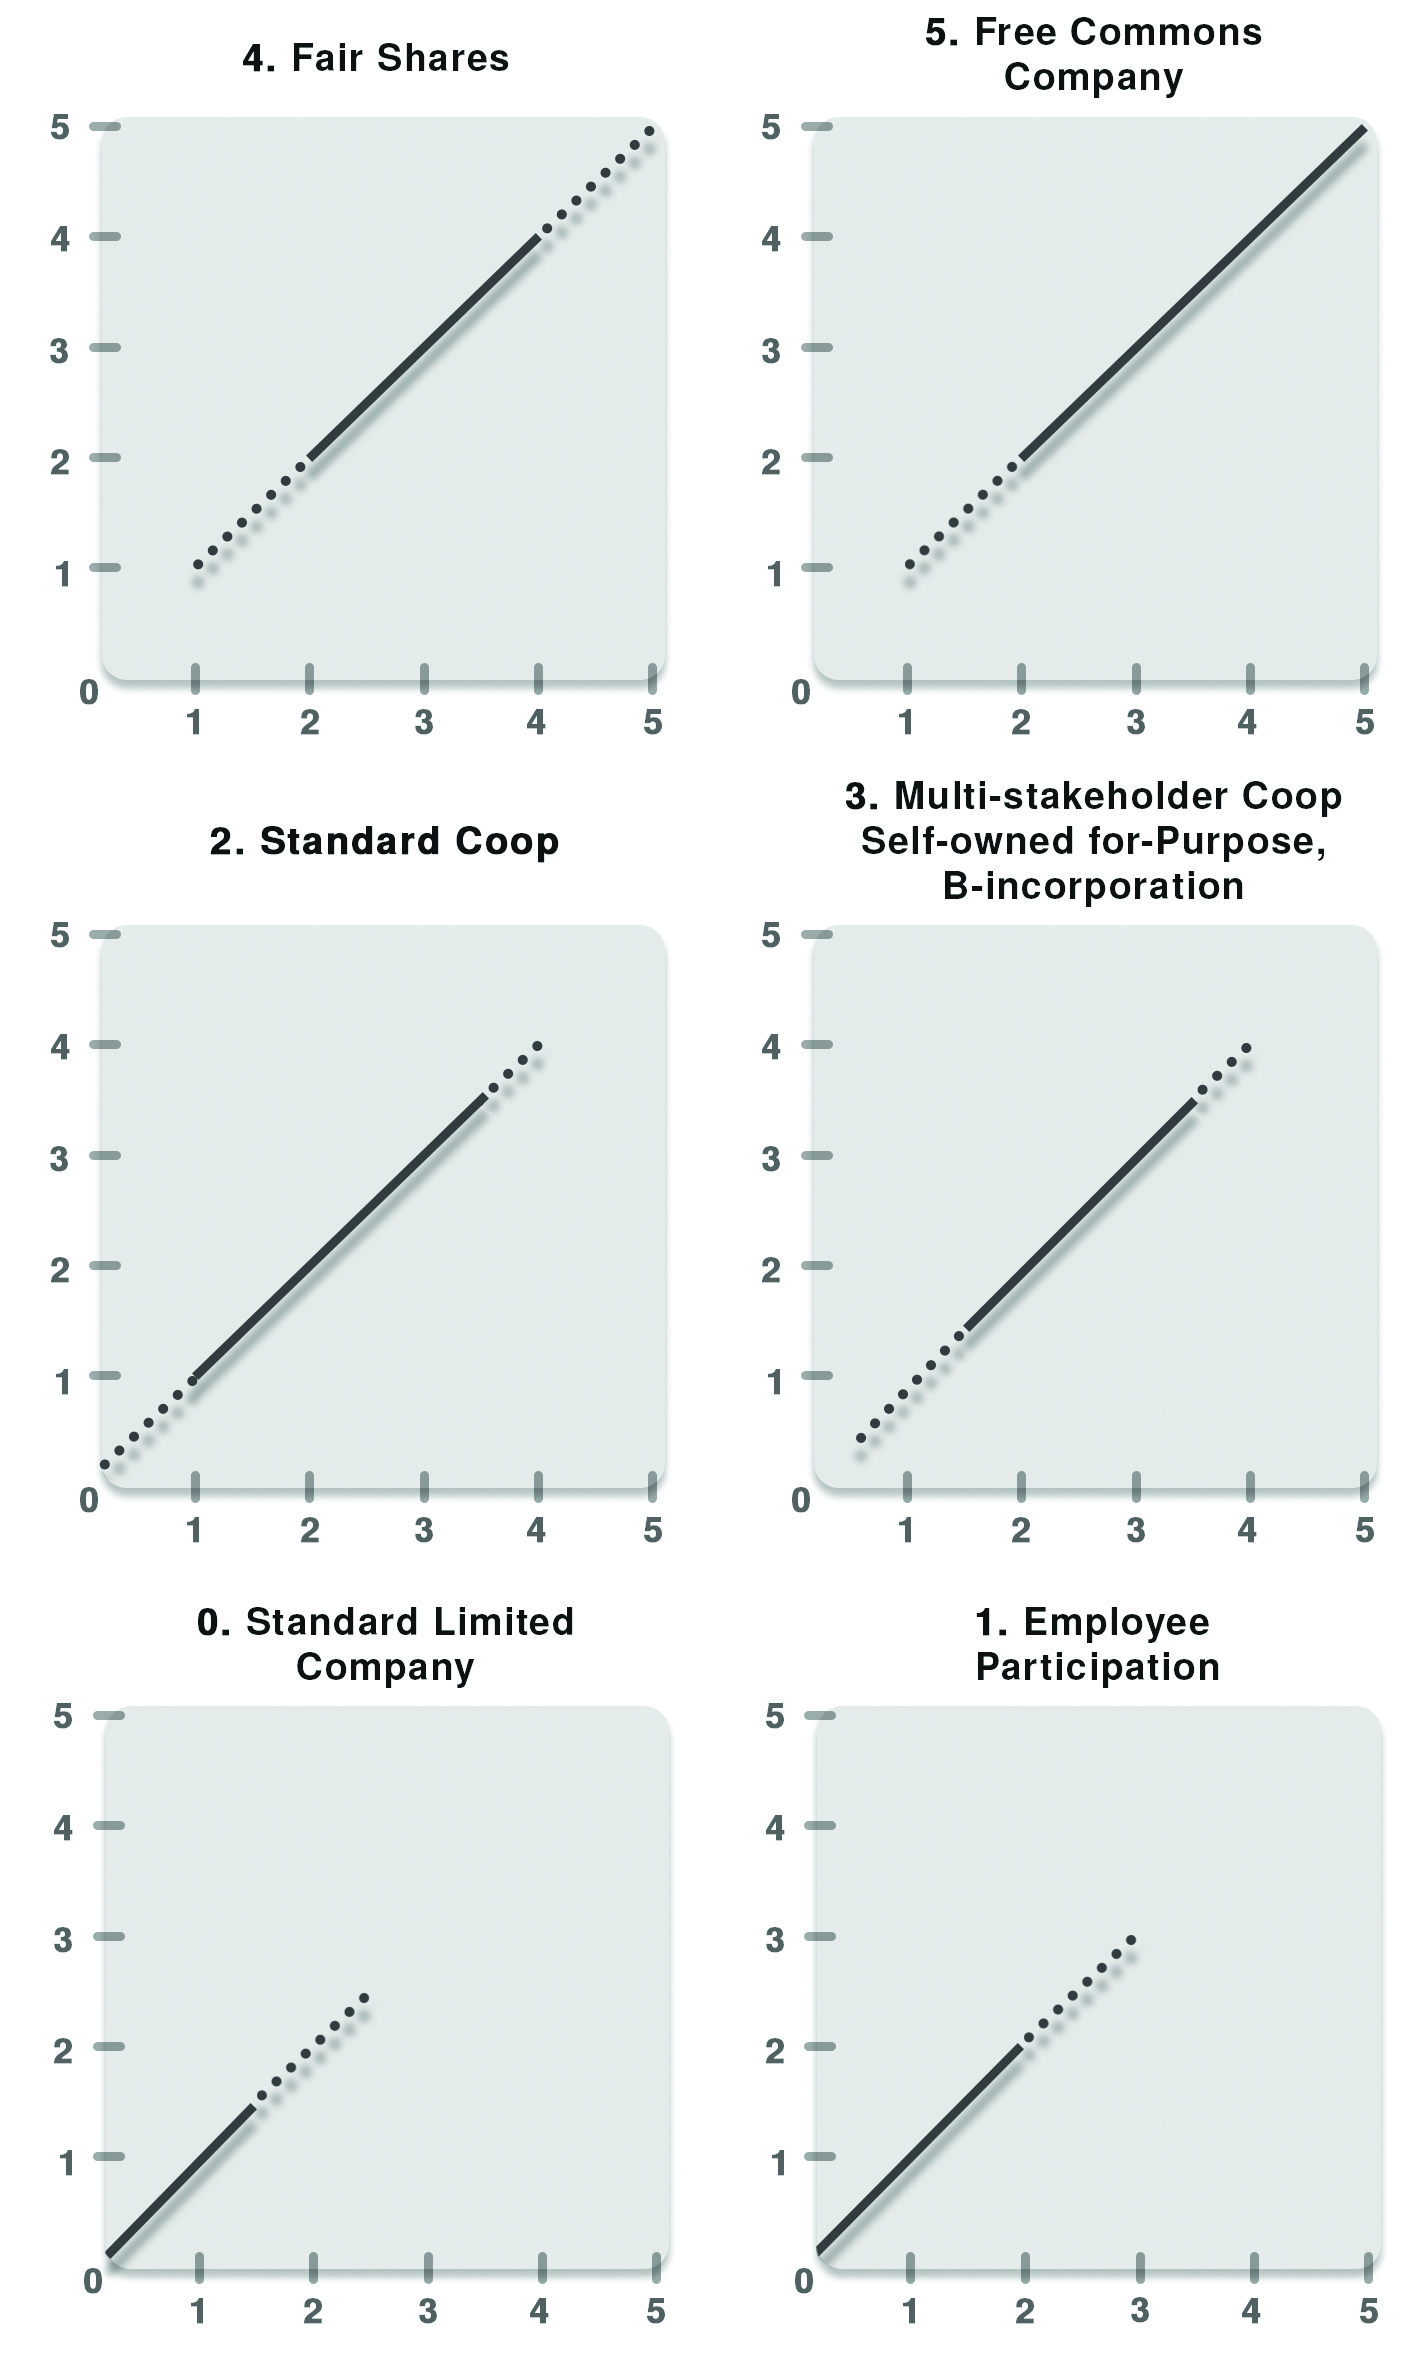
\includegraphics[width=0.75\textwidth]{./Images/stable-valley}
\caption[Stable valley for growing your organisation to Level 555.]{The valley of continuous stability as organisations grow their capacity along the two axes of human development and organised task execution. Each square shows the viable valley for that level of incorporation. Solid diagonals represent systemic stability, dotted lines fragile stability dependent on the leadership to maintain.}
\label{fig:SDO-valley}
\end{figure}


This valley has good news for you, whatever type of organisation you are in. There is a simple small next step you can take, deeper along the valley, wherever you are now. Even a Management Accountability Hierarchy \index{Management Accountability Hierarchy}lying at the bottom left can easily introduce simple Adaptive Way \index{Adaptive Way} patterns, like giving effective feedback, and take a step towards becoming a developmental organisation. You can introduce simple self-management patterns that take you a step towards becoming self-organising. 


Each little step will bring benefits, and ease taking the next step, up to the limit of what your incorporation can sustain.


If you have already stepped far along the self-governing organisation direction, pay vigilant attention for any signs of stepping beyond what the current meaning\hyp{}making stories can support, or beyond what your organisation's developmental stage can keep within everyone's Zone~3. 


It is very easy for an ambitious change agent to lead, without realising until it is too late, that their organisation has gone too deep into self-organising, forcing people into their Zone~4. This is the panic zone, where you cannot perform regardless of how much support you have from both the organisation and outside, and all you can do is either shut out what is so far beyond your Size of Person, \index{Size of Person} or leave. 


Either way, you are likely to be highly stressed and harmed, and equally so the organisation. 


Everyone in your organisation will be best served if they are all fluent in the Adaptive Way patterns, at the very least in the Ground Pattern and the first few in each category of the 28 thought forms. \index{thought forms (28)} 


Once everyone is fluent, you are far on a journey towards becoming a developmental organisation. To reach the highest levels as a development organisation you also need the power of self-organising.  


If you are a change agent, or the CEO leading the transition away from a person-centred hierarchy and shifting a company towards Holacracy, you have a make-or-break role in developing this adaptive capacity in every individual and team. Best to do it by introducing structured patterns of dialogue, so that it happens as part of work, at no extra cost, time, or effort.


Your job leading change spans all four layers. You will be supporting individual social-emotional and cognitive development; interactivity and reciprocal helping; self-governing organisation design and processes; requisite matching of task to individual; and changing the shareholder structure to one that enables and doesn’t hinder this. 


So developing high performing teams, whether in a traditional company or modern self-governing teams (circles, as they are more commonly called) demands far more than has ever before been expected of a team coach, employee or leader today. 


\subsection{Divided teams}
\index{teams!divided}
\label{section:divided-teams}
Organisations are intended to be good at chunking down\footnote{Taking a role, or task, that is too big to do and breaking it down into smaller ones (chunks) that can be done.} the complexity of roles, but sometimes the complexity is inherent and irreducible. When it is, you cannot divide it down into simplicity. Whoever fills these roles must be big enough to grasp the full complexity. 


Also, anyone within a team or circle who has a smaller SoP than the whole team’s SoR \index{Size of Role} may cause the entire team to function at a lower size than required for its task.


When a team, or circle in an Ocracy,\index{Ocracy} needs to take a decision, the team as a whole must be at least as big as the entire driver and decision. So either every single member must have a big enough SoP, or each member must be psychologically able to recognise and take a decision they have not fully grasped. 


Most teams have a few members at a bigger or smaller SoP than the team centre of gravity. This is called a divided team, and has important implications for how the team can rise to their largest challenges, especially adaptive ones. 


In trying to understand who your organisation \index{organisation} is, the first question you should ask is whether the team leader or lead link has a bigger or a smaller SoP\index{Size of Person} than the team's centre of gravity. If it’s bigger, and they have sufficient respect from the rest of the team, they will be able to provide the developmental scaffolding to support the whole team to take decisions that are bigger than its average SoP.


However, if their SoP is smaller than the centre of gravity, you had better hope that the team leader has the humility to follow the team. I have so often seen team leaders who have a smaller SoP than the people they are leading, but have the formal or personal power to overrule the others in the team. This leads eventually to the team taking overly simplistic decisions that cannot reliably help the business to survive, let alone thrive.


Usually only an outsider with a sufficiently bigger SoP than any individual in the team can recognise which way round it is divided, because of the Dunning-Kruger effect. \index{Dunning-Kruger effect} The team itself, and its members, unless they have proficiently applied everything in this book, probably won’t be able to tell the difference.


The ideal team, or Ocracy circle, is composed of people of more or less the same size. This ideal is rare in any team bigger than three people. More normally the team is divided. And then you need to have interpersonal relationships and psychological safety such that the team as a whole takes decisions at a SoP = SoR, regardless of the SoP \index{Size of Person} of whoever has formal authority over the team or decision domain.


In such a divided team, the few individuals with a larger SoP than the team's centre of gravity are recognised and explicitly tasked by the team with growing everyone's SoP.


\section{Sociocracy, Holacracy, etc.}
Sociocracy and its various forks emerged from the philosophy of Auguste Comte. \index{Comte, Auguste} He recognised that governance in modern society could no longer be based on inherited or appointed power. Thus was born the philosophy of sociocracy, which loosely translates as \emph{society governing itself}.


The first practical implementation of the sociocratic philosophy in an organisation was in a school in the Netherlands, founded by Kees Boeke and Beatrice Cadbury Boeke during the Second World War. 


Since then an ever-growing number of organisations have recognised that being at an appropriate level along the journey towards full self-organising, appropriate for their business context, increases their business results and staff well-being.


Ted Rau, \index{Rau, Ted} co-founder with Jerry Koch-Gonzales \index{Koch-Gonzales, Jerry} of \emph{Sociocracy for All (SoFA)} and authors of an excellent book on implementing sociocracy, \emph{Many Voices, One Song}\cite{rau-sociocracy}, describes it well in the following guest contribution.
\begin{longstoryblock}
Since we spend so much time in organizations, why not make them a place where we can thrive as humans, and contribute positively to the world we want to live in? 


The founder of sociocracy in its modern guise, Gerard Endenburg, \index{Endenburg, Gerard} a former student of the Boekes’ school, sees the essence as \emph{no one ignored}. SoFA translates that into \emph{everyone's needs matter} and \emph{everyone’s voice matters}.




Sociocracy is a practice of equality and it can have a positive impact on everyone.


\begin{itemize}
\item It creates space for personal growth because you have self-responsibility and trust-filled relationships with others.
\item We can meet people’s needs through organizations, including autonomy, competence, relationships, contribution, belonging, and meaning. 
        \end{itemize}


Sociocracy\index{Sociocracy} is \emph{one} framework of many that allows us to hold complexity while generating more ability to act in ways that are healthy for us and the planet.  
\end{longstoryblock}


And at the same time many early adopters of self-managing, self-governing, or even self-organising, methods added their own flavour to what they do. So now you have a wide range of approaches, including Holacracy\cite{robertson-holacracy}, sociocracy\cite{rau-sociocracy}, and Sociocracy~3.0\cite{priest-s3-web,cumps-sociocratie}, with close relatives in the agile approaches. 


All have value, all have advantages and disadvantages in specific contexts, and all have passionate adherents. 


One challenge some transitions to an Ocracy face, that this book addresses: whenever anyone in an organisation still has S3 elements to their meaning making, they must either have actual people as role models creating new norms for the group, or become part of a large group that already consistently practices these norms. 


This means that in any organisational change journey, the role of real live human beings in shaping the group's meaning making (lower left), and the meaning making of each person (upper left), can never be fulfilled by structures and processes (integral lower right). 


There are now a large number of excellent websites and books filled with everything you need to build your own unique flavour of Ocracy, \index{Ocracy} or to apply one of the existing approaches, so I’ve not repeated what others have already done better. 






\section{Task and role arena}
Here I touch briefly on how to build the structures and processes your organisation needs for tasks and roles, integrated with the other three layers of an Adaptive Organisation:  intra-personal, inter-personal, and stakeholder incorporation. 


After all, to actually get many people to work together does require some way of organising tasks and roles, and some way of mining and refining conflict and tension, in order that the organisation continuously improves its fit with the external drivers whose need it exists to meet\footnote{
Specialist books about each approach include: Sociocracy in \emph{Many voices, one song}\cite{rau-sociocracy} by Ted Rau\index{Rau, Ted} and Jerry Koch-Gonzalez; Holacracy in Brian Robertson’s\cite{robertson-holacracy} book; and Sociocracy~3.0, \cite{priest-s3-web} by James Priest, Bernhard Bockelbrink, Liliana David and many others in the S3 community\cite{cumps-sociocratie}. Books on the theme of creating such organisations include Frederic Laloux's \emph{Reinventing Organisations}\cite{laloux-RO,laloux-illustrated} and \emph{New work needs inner work}\cite{breidenbach-new}. There is much more, e.g., Appreciative Inquiry and Open Space Technology; the Chaordic Organisation approach developed by Dee Hock;\index{Hock, Dee} Decentralised Autonomous Organisation (DAO); and the Open Organisation. There are so many good approaches out there that it's best for you to choose what seems right for you and your organisation in your current context.
}. \index{Reinventing Organizations} \index{Laloux, Frederic}




\subsection{Minimum viable structures and processes}
Recall that I regard an organisation as living, as represented by Wolfe’s \index{Wolfe, Norman} equation, $P = [ A \times R^{2} ]^C$. I find looking at the smallest unit of an organisation, the human being, a good model for the journey of an organisation.


When you were first conceived, you were one embryonic cell, somewhat like the founder and source of a startup. Then you were two cells, and then four. At this stage, none of your cells had distinct roles, and there was no hard structure like a skeleton. All four cells were simultaneously taking care of themselves, each other, and the whole. 


As the number of cells grew, the minimum viable level of differentiation in roles, and the minimum viable structure, was implemented to fit the needs of each stage of growth. Your body grew with amazing speed and efficiency, extracting the most results from the least investment in structure.


At some point you were born, and even then the structure of your skull had not yet reached its final shape. You grew in size and complexity. Your brain only reached full adult complexity around the age of 25. Your Size of Person \index{Size of Person} continues to grow long after that.


All the distinct growth stages you went through were exactly right to give you just enough structure for you to maximally adapt to the life conditions you were in at the time, and to get your energy flowing. 


The same applies for any business as a living being. Your topmost priority is to maximise the free energy\index{energy!free} available to convert into business results. That needs all the capitals to be present in viable quantities and flowing. Build the right organisational structure for the stage you are entering.


After all, the first liver cell in your body did not have the full structure of veins and arteries of an adult liver. Avoid building a highly developed structure before you are close enough to needing it. 


Energy flows when, where and how it wants to flow. The very essence of your organisation, because it is a living being, is the nebulous, unknowable, and uncontrollable energy flowing and transforming into business results. Just the right amount of structure and process definition is needed to maximise energy flow and conversion into output. Keep a very careful eye on where energy\index{energy} is and isn’t flowing, and adjust what is happening to get it flowing and converting everywhere.


Also keep in mind what we covered in Section~\ref{section:integral-organisation}. The workplace reality that you experience is your inner workplace, not the tangible outer workplace. Work with all quadrants in Figure~\ref{fig:integral-organisation} to bring your organisation to life. There are a number of approaches that have proven very useful in creating minimum viable structures in organisations. You will find a number in these references\cite{aoh, possert-playbook, ganescu-playbook, lipmanowicz-liberating, breidenbach-new}.


\subsection{Multiplicity of roles}
In every organisation\index{organisation}, everyone plays a multiplicity of roles. In an Adaptive Organisation\index{Adaptive Organisation}, this multiplicity is made explicit, so that you can play these roles with full recognition and support from your colleagues and organisation. 


In an Adaptive Organisation all members of staff are simultaneously executives, workers, leaders and followers. Even more so, as you'll see in the next section, customers, suppliers, family members and the community you live in may also be executives, workers, leaders and followers for your company.


Making this explicit means that nobody is disempowered from interacting wherever and however they can add value to the organisation. It also means that the organisation can expect everyone to be an effective executive and care for the whole organisation as a meaning\hyp{}making living being, whatever your most primary role or stakeholder category is.


It means that the newest hire's, or the most junior person's perception, of what the organisation needs from its people must have a systemic place to be heard. In addition to any visible, explicit role you may have in the organisation’s lower right quadrant (either a Management Accountability Hierarchy \index{Management Accountability Hierarchy} or a  Functional Accountability Hierarchy), \index{Functional Accountability Hierarchy} you and everyone else always has a number of hidden, implicit roles in your organisation’s lower left quadrant (Human Capability Hierarchy).\index{Human Capability Hierarchy}


Think about this perspective in a meeting, for example, a governance meeting. It is clear that you are always sitting there with both explicit and implicit, visible and hidden organisational roles. You may feel a tension in one of the explicit MAH/FAH roles that the meeting is explicitly about, you may feel a tension in one of the implicit HCH roles, or even in both. This is the same as quantum mechanics: what you see when you look at the roles is not the same as what the roles actually are. 


The better scaffolding is enabling you to speak as clearly as you can to bring the tension into the meeting so that everyone can mine and refine it,  the better the organisation\index{organisation} is at being fully adaptable.


Keep in mind that the most pivotal tensions often begin as a nebulous feeling, pointing at a deeply hidden tension, not yet open to any articulation, let alone one that anyone else is able to see sense or logic in. The single most important tension to mine and refine may well be the one that cannot be articulated any more clearly than someone simply saying 


\begin{quote} 
I feel a tension listening to this proposal. Something doesn't feel right, and I cannot articulate what it is. I request \ldots ( time / a sparring partner / discussion and debate on) to get to a point where we can articulate something more clearly.  
\end{quote}


\subsection{Are executives born or made?}
Since everyone needs to be effective in all roles, both explicit and implicit, part of your journey in an Adaptive Organisation is to continuously increase everyone’s effectiveness. 


Peter Drucker came to the conclusion that effective executives are made, not born. He found that every single top executive who he met had had to learn how to be effective. Every single one had had to learn how to be more subtle with ineffective elements of their nature, biases, and meaning\hyp{}making stories. His excellent short book, \emph{The Effective Executive}\cite{drucker-eff-exec}, albeit written in the 60s, is as relevant in an Ocracy of today as it was in the Management Accountability Hierarchies that predominated when he wrote it. Peter Drucker was, in my (Graham’s) opinion, one of the pioneers of today's trend towards Ocracies\index{Ocracy} and the Adaptive Organisation.\index{Adaptive Organisation}


Drucker\index{Drucker, Peter} has summarised the common characteristics of effective executives.


\begin{enumerate}
\item  They ask \emph{what needs to be done?} Which means they stand more often in a place of ignorance and curiosity, not in a place of certainty; and actively keep looking at the context and needs for anything new or changing.
\item They ask \emph{what is right for the enterprise?} Doing this well requires fluidity in all thought forms, especially C6 (Frames of Reference).
\item They develop action plans. How and what they do here depends on where the organisation is, in the categories of Section~\ref{section:where-is-your-organisation-tasks}.
\item They take responsibility for decisions. Regardless of which category your organisation is, taking responsibility for decisions in your domain is the minimum. And in any HCH or FAH you always have a decision domain.
\item They take responsibility for communicating. This applies to any and everyone in any organisation. You are all executives in many senses.
\item They are focused on opportunities, rather than problems. For many people, this is a big challenge. Problems are usually so much easier to lay out clearly, and have clearer ways of solving them. Opportunities are often inherently nebulous.
\item They run productive meetings. Well, yes.
\item They think and say we, rather than I. This is an art, not a science. It is all about the art of facilitating human beings to bond together, to feel energised, and to engage in the reciprocal helping that creates the collaboration needed for high team performance. So sometimes it's important to say I, and at other times it's we.
\end{enumerate}


Of course, his work ought to be read together with complementary work, say by Margaret Wheatley\cite{wheatley-leadership,wheatley-lost-found} which played a pivotal role in my (Graham) journey towards this book. And keep in mind, where you find contradictions between them, that the opposite of a deep truth may be another quite different deep truth. 
\subsection{UniOne and nebulous}
Of course, the characteristics of being an effective executive in an Adaptive Organisation\index{Adaptive Organisation} have some important nuances. The most important is that in an Adaptive Organisation we inherently recognise that much is nebulous and cannot be pinned down, because the organisation is inherently in both lower left and lower right quadrants. These quadrants are complementary pairs, as in quantum mechanics.


An Adaptive Organisation, for example, harnesses both the uniqueness of each individual and the common oneness of everyone\textemdash the full complementary pair\textemdash to be truly one living organisation and part of one business ecosystem. (Read more on creating living regenerative business ecosystems \index{ecosystems} in Section~\ref{section:incubating-regenerative-ecosystems}.)


In a traditional vertical hierarchy, the dominant meaning\hyp{}making stories are likely to be concentrated on individual uniqueness. Stars will be disproportionately fêted and rewarded (even though the research that you read about in Sections~\ref{section:interactivity} and~\ref{section:coming-together} proves that the star’s success is primarily a consequence of the whole organisation in which they are embedded).


So in these organisations, the most long-term effective executives are those who explicitly restore the natural balance between uniqueness and oneness that characterise any living being. They say \emph{we} far more often than \emph{I}. 


In an Adaptive Organisation, \index{Adaptive Organisation} you need to work out when it will serve best to emphasise the uniqueness that you or a colleague brings\textemdash then say I. Or, if it serves the organisation better to emphasise the common oneness\textemdash for example, to note the common ground that you are all standing on as representatives of this living being\textemdash say we. 


During the course of my working life, I (Graham) have been criticised almost equally for using I, and for using we. You most likely will be too. Every single criticism had validity, as had my choice in the first place. This is another classic example of the nebulous, quantum, or Cubist essence of an organisation. I can always speak with the voice of we because I am part of what is common to all of us and represent it just as much as any other individual can represent oneness from within their own unique meaning\hyp{}making and reality. 


Equally, each person criticising me could only experience my words in terms of their own unique inner reality.


The more comfortable everyone is with the nebulousness of organisations and language, the easier it gets to hear the intent behind the words and to choose words that make that intent easier to hear. As with any Picasso\index{Picasso, Pablo} painting, both the painter and the viewer jointly shape what the viewer sees in the painting, or hears in the words, or perceives in the actions.


Seeing an organisation as a living being, filled with nebulous complementary pairs that cannot individually and simultaneously be pinned down precisely, requires equal effectiveness in head and heart. Equal effectiveness in using conscious thinking (especially transformational thought forms, not just binary logic) and using intuition. And equal effectiveness in applying hard empirical data, and crossing unknowable chasms using nebulous clouds of intuition as your stepping stones.


As Einstein said, 
\begin{quote} 
Not everything that is important can be measured, and not everything that can be measured is important. \index{Picasso, Pablo}
\end{quote} 


Or as Peter Drucker \index{Drucker, Peter} points out, data is not the foundation of your data-based business decisions, opinion is. 


You begin with an opinion, likely anchored in your intuition (i.e., anchored in your biases, nature, and meaning\hyp{}making stories; limited by your capacity for transformational thought forms). An opinion on what you are dealing with, and so what kind of data will be useful to you in generating useful options to choose between, and driving your choice. This opinion is created and limited by your Size of Person. Any data that does not fit within this Size of Person \index{Size of Person} you won’t look for; and, if it is given to you, you may not be able to fit it into your reality.


Very few of us are equally and sufficiently good in intuition and thinking\textemdash most of us are naturally more talented in one or the other. If your natural talents lie predominantly in the visible explicit lower right MAH/FAH, then you need to develop your comfort with aspects of your organisation that you may well find highly uncomfortable. Find a colleague who is naturally talented in this area, and a route for both of you to use the tension between your natural talents to then develop into two legs that your organisation can run with; rather than you trying to be one single super leg that your organisation can only hop with.






\section{Scaffolding to stay out of the panic Zone~4}
Deploying the scaffolding\index{scaffolding} described here will benefit all organisations, but it is essential for any organisation aiming to become Level 5 in each three axes of the Adaptive Organisation\index{Adaptive Organisation} model. To determine what scaffolding is needed, by whom, and when, ask two questions.


\begin{enumerate}
\item With which SoP\index{Size of Person} do circle members, individually and collectively, put their competencies to work?
\item Therefore, what Job~2 supports do the work structures and processes need to provide, individually and collectively, in the three elements of Size of Person?
\end{enumerate}


The work of a leader, change agent or coach, anyone with a lead link role, etc., goes beyond what is typically expected of a team coach today because people are challenged at many levels by the identity paradox created by working sometimes as a peer, then above, and then below the same colleague. Leaders work now spans all six layers of Section~\ref{section:harnessing-conflict-intro}, at least the first four layers described in Section~\ref{section:adaptive-organisations}. 


In any organisation, management, or the anchor circle and lead links, has the accountability to both construct this scaffolding and to match the Size of Person\index{Size of Person} to the Size of Role \index{Size of Role}. This is an absolute imperative in an Adaptive Organisation. \index{Adaptive Organisation}The anchor circle (i.e., equivalent to the leadership team in a traditional organisation) and, to some degree, everyone, works constantly on constructing the scaffolding that the circles use on a day to day basis.


For each developmental stage a different scaffolding \index{scaffolding} is needed. 


\begin{enumerate}
\item In Zone 1, continue to do what any good organisation does for each stage.                  


\begin{itemize}
\item S3: clarity on the expectations of physical others, and feedback from them. (NB: this needs to be physical others, just role clarity fails to deliver what the meaning\hyp{}making identity needs.)
\item S4: roles where you act according to your personal values. 
\item S5: fully developmental and self-organising in your immediate organisation space.
\end{itemize}


\item In Zone 2, where work requires individuals to stretch up into their current growth zone, you can then usually self-support given the above. You are at your best if you also have


\begin{itemize}
\item S3: strong personal bonding with other circle members.
\item S4: alignment, clarity and buy-in to the big picture across all peers. 
\item S5: roles demanding constant stretching, growth in maturity and flexing of your full meaning\hyp{}making range.
\end{itemize}


\item In Zone 3, work requires a size beyond your capacity to self-support, but you can act if given sufficient support from the organisation's structures and processes, and your colleagues. 


\begin{itemize}
\item S3: you need peer to peer coaching practices you fully trust in, and that all your peers also use effectively. Processes that are the cultural norm and expectation, not just policy.
\item S4: a peer group of individuals that you recognise as being of equal or larger Size of Person to yourself, and so you trust them as human beings to be able to give you useful feedback on your integrity and value system. Others may give you feedback that you deem useful.
\item S5: Peer to peer exchange of a deeply mutually developmental nature
\end{itemize}


\item In Zone 4, the size required is completely beyond you. No scaffolding exists. 
\end{enumerate}


In Section~\ref{section:public-agreements} we described how public agreements\index{public agreements} are one type of scaffolding. Hopefully this section makes more clear the imperative of using such scaffolding whenever your organisation brings in Holacracy, Sociocracy or any other self-governing approach.


Since this support must be an integral part of all work processes, a peer-to-peer developmental scaffolding is needed for any self-governing organisation design to truly work. Any organisation benefits, of course, whether agile or even a traditional management accountability hierarchy. But as long as a self-governing organisation lacks the capacity to change the organisation design at all scales, such peer-to-peer developmental scaffolding\index{scaffolding} will always be less effective.